%\documentclass[fleqn]{book}
\documentclass[11pt]{amsbook}

\usepackage[turkish]{babel}

%\usepackage{../HBSuerDemir}	% ------------------------
\usepackage{../Ceyhun}	% ------------------------
\usepackage{../amsTurkish}


\begin{document}
% ++++++++++++++++++++++++++++++++++++++
\hPage{226}
% ++++++++++++++++++++++++++++++++++++++

\begin{figure}[htb]
	\centering
	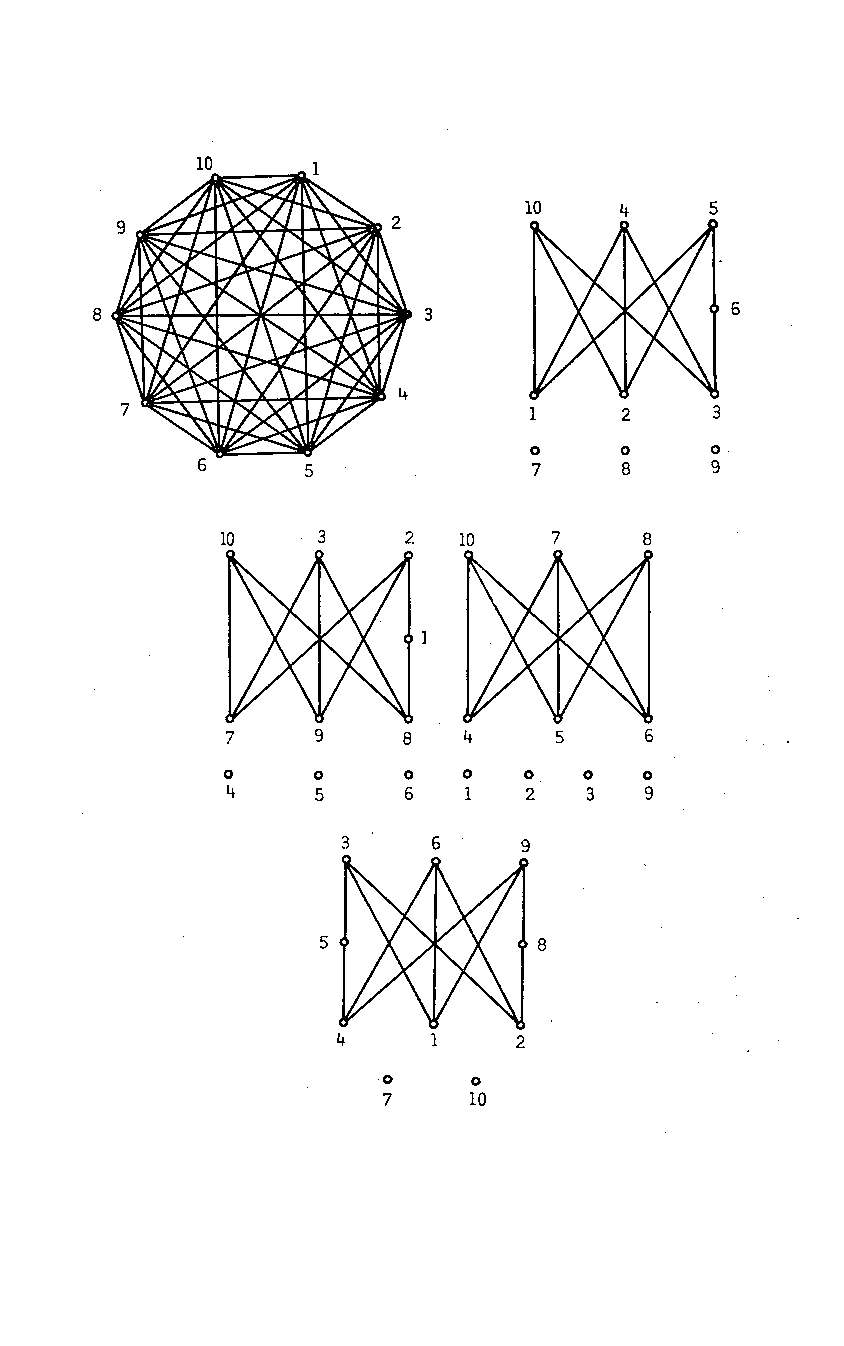
\includegraphics[width=0.75\textwidth]{images/ceyhun-226-fig01.pdf}
	\caption{Kalabalığı 4 olan $D(10)$ çizgesinin düzlemsel olmayan çizgelere ayrışımı.}
	\label{fig:Ayrisma}
\end{figure}
    
\end{document}